\chapter{Introduction}

Richard Feynman originally suggested the idea of a quantum computer in a 1982 article\cite{feynman_simulating_1982}, demonstrating that current computers experience an exponential slowdown when simulating quantum physical systems. In this paper, he proposes using a different type of computer: one that runs according to the laws of quantum physics, to simulate quantum physical systems without a slowdown.\cite{Hirvensalo}

\section{Computational models}

The current computational model we use for classical computers is called the Turing-machine. These new types of computers are so different from classical ones that they run based on a completely different set of rules. Following the work of many computer scientists (Benioff\cite{benioff_models_1998}, Deutsch\cite{deutsch_quantum_1985}, and Bernstein and Vazirani\cite{bernstein_quantum_1993}), the computational model for Quantum computers was mathematically defined in the late 1980s: the Quantum Turing machine.

In the classical world, on the Turing machine, mathematicians and computer scientists have been working on coming up with fast solutions to all kinds of algorithmic problems. Many of these problems have important real-life applications, but nobody has been able to come up with a fast solution to them. A subcategory of these unsolved problems is the ones where at least we are able to verify in a fast manner if a solution is correct, these are called the 'NP' problems. A simple way to use the verifier algorithm to solve a problem is to look at all of the possible solutions (the domain of the problem) and verify every one of them, until we find a correct solution. This runs in $O(N)$ linear time relative to the size of the problem's domain. The question is, can we do something faster? This is one of the famous Millennium Prize Problems set by the Clay Mathematics Institute a hundred years ago, the P versus NP problem. This problem has eluded computer scientists for a century.

In the quantum world, on the Quantum Turing machine, there exists a better method for the classical linear verifier search, which can do it in $O(\sqrt{N})$ time, relative to the size of the problem's domain. This algorithm is called Grover's search. It has also been proven by Bennett, Bernstein, Brassard, and Vazirani, that this is asymptotically tight\cite{bennett_strengths_1997}.

\section{Application of quantum algorithms in bioinformatics}

An interesting area for algorithmic research is bioinformatics. Many problems here have significant impact on our everyday lives since discoveries in this area can help us solve many of today’s major global problems, for example, aiding the creation of more effective medical treatments, advancing our understanding of genetic diseases, developing resistant crops to tackle a global food crisis or inventing novel technologies to reduce and revert environmental pollution. I am particularly interested in computer-aided drug design, where problems such as protein folding\cite{crescenzi_complexity_1998} and molecular docking\cite{a_molecular_2018} turn out to be NP-hard ones, which means that despite decades of effort, we have yet to come up with efficient solutions to them using classical computers.

In the past year I have been researching protein folding and how to implement it on a general-purpose quantum computer. I have ran into a significant problem: I was unable to run any experiments of usable size, mainly due to limitations in memory. Due to quantum parallelism, the memory requirements of running a quantum calculation simulation are super-exponential. In particular, there is one component in Qiskit, which seemed to come back in any form of model I have tried to implement: a quantum gate for taking the sum of $n$ qubits, called the WeightedAdder class. 

This component came to my attention, because a natural way to encode protein structures is by creating a 2D or 3D grid and laying the aminoacid chain down on it\cite{dill_principles_2008}, as seen below.

\begin{figure}[H]
    \centering
    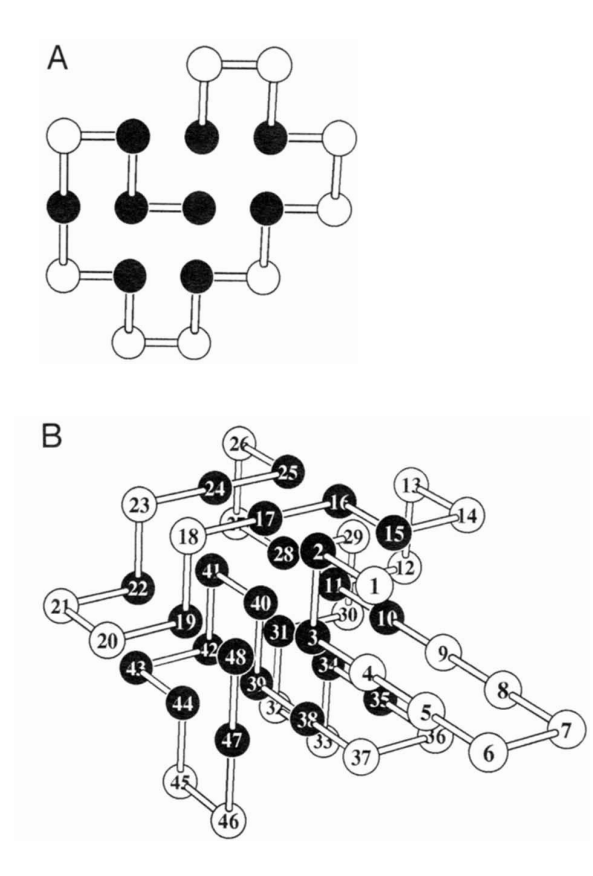
\includegraphics[width=0.5\linewidth]{figures/bioinformatics/hp_model.png}
    \caption{HP model of protein folding\cite{dill_principles_2008}}
\end{figure}

From a single vertex in a 3D grid, we can step in $4$ or $6$ directions: up, down, left, right and inwards and outwards in the 3D case. We can encode these naturally, using one-hot encoding, by introducing $6$ bits of information. If we assume that the chain starts in the origin, then we can encode a chain shape by giving the directions of the $(n-1)$ steps it takes.

A chain like this is viable, when it doesn't cross over itself. A chain's optimality is assessed by counting how many pairs of various aminoacids are neighbouring each other. To answer both of these questions, we must be able to calculate relative distances between any two points of the chain. Using the directinal one-hot encoding model, these questions can be answered by taking the sum of some qubits.

Using these operations, we can create a quantum oracle, that assesses the optimality of a particular chain and use Grover's quantum search algorithm to find the best possible solution.

Unfortunately, while Qiskit itself is open-source, it's architecture (similarly to other quantum computing frameworks) is designed from the core to store the matrices of various operations (such as the WeightedAdder operation) in its memory and retrieve this information during simulation. This means that I am unable to correct this single operation in Qiskit.

\section{Contents of this dissertation}

In order to reduce the memory requirements for any quantum computation simulation, I have to be able to reduce storing large operation matrices in memory whenever I can. This requires a completely different architecture.



\section{Contents of this dissertation}

\subsection{TDK 2021/Dipterv}

The rest of this thesis is structured in the following way: In Chapter 2, I introduce Quantum computing, specifically Quantum Random Walks, in a bottom-up approach, starting from the simplest form and then generalizing it. Contrary to many authors, I use linear algebra exclusively to describe each step since implementation on a universal quantum computer requires the definition to come in the form of unitary transformations.

Section 2.2.5 discusses two of the generalization techniques found in~\cite{Portugal}. I present my improvement to one of these methods, which I have proven to have the equivalent result but remove an exponential memory requirement from the implementation. The other method in~\cite{Portugal} uses a constraint about the evolution operator, for which I have not found proof in the literature. Here, I present my more generalized version of this constraint and the proof I have given.

In Chapter 3, I introduce three bioinformatics problems: DNA sequencing, Protein folding and Molecular docking. I explain the computational models that emerge from these practical problems and the well-known computational problems they reduce to.

In Chapter 4, I describe my simulator software's architecture and implementation details and present the results obtained from my simulation runs.

\subsection{TDK 2022}

The remaining chapters are structured as follows: In Chapter 2 I introduce Grover's search algorithm framework and solve a generalized version of the Sudoku puzzle with it. I iterate over the necessary components from this solution, the particular operators needed for the oracle and the amplitude amplification technique's implementation. In Chapter 3 I lay down the mathematical foundations for a quantum simulator framework's implementation, particularly the solution to applying a quantum operator to a subset of the registers in the system, then I introduce the quantum operators and their implementations in my system. Finally, I describe the architectural design patterns used in the system. In Chapter 4 I summarize the results of this paper and lay down my plans for the future.